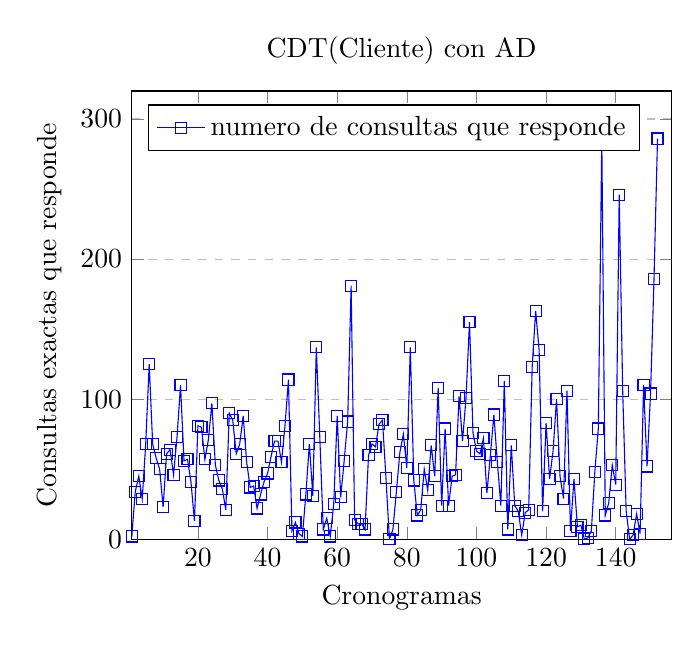
\begin{tikzpicture}
\begin{axis}[
    %CDT = carga de trabajo
    %AEPxT = Algoritmo DETERMINISTA
    title={CDT(Cliente) con AD},
    xlabel={Cronogramas},
    ylabel={Consultas exactas que responde},
    xmin=1, xmax=156,
    ymin=0, ymax=320,
    xtick={},
    ytick={},
    legend pos=north west,
    ymajorgrids=true,
    grid style=dashed,
]

\addplot[
    color=blue,
    mark=square,
    ]
    coordinates {
   %CARGA DE TRABAJO CLIENTE
   (1,2)
(2,34)
(3,45)
(4,29)
(5,68)
(6,125)
(7,68)
(8,58)
(9,50)
(10,23)
(11,61)
(12,64)
(13,46)
(14,73)
(15,110)
(16,56)
(17,57)
(18,41)
(19,13)
(20,81)
(21,80)
(22,57)
(23,71)
(24,97)
(25,53)
(26,42)
(27,36)
(28,21)
(29,90)
(30,85)
(31,61)
(32,68)
(33,88)
(34,55)
(35,37)
(36,38)
(37,22)
(38,32)
(39,41)
(40,47)
(41,59)
(42,70)
(43,70)
(44,55)
(45,81)
(46,114)
(47,6)
(48,12)
(49,4)
(50,2)
(51,32)
(52,68)
(53,31)
(54,137)
(55,73)
(56,7)
(57,15)
(58,2)
(59,25)
(60,88)
(61,30)
(62,56)
(63,84)
(64,181)
(65,14)
(66,11)
(67,11)
(68,7)
(69,60)
(70,68)
(71,66)
(72,82)
(73,85)
(74,44)
(75,0)
(76,7)
(77,34)
(78,62)
(79,75)
(80,51)
(81,137)
(82,42)
(83,17)
(84,21)
(85,50)
(86,35)
(87,67)
(88,45)
(89,108)
(90,24)
(91,79)
(92,24)
(93,45)
(94,46)
(95,102)
(96,70)
(97,101)
(98,155)
(99,76)
(100,63)
(101,61)
(102,72)
(103,33)
(104,60)
(105,89)
(106,55)
(107,24)
(108,113)
(109,7)
(110,67)
(111,24)
(112,20)
(113,3)
(114,19)
(115,21)
(116,123)
(117,163)
(118,135)
(119,20)
(120,83)
(121,43)
(122,63)
(123,100)
(124,45)
(125,29)
(126,106)
(127,6)
(128,43)
(129,9)
(130,10)
(131,0)
(132,1)
(133,6)
(134,48)
(135,79)
(136,285)
(137,17)
(138,26)
(139,53)
(140,39)
(141,246)
(142,106)
(143,20)
(144,0)
(145,3)
(146,18)
(147,4)
(148,110)
(149,52)
(150,104)
(151,186)
(152,286)
    };
    \legend{numero de consultas que responde}

\end{axis}
\end{tikzpicture}